
%%%%%%%%%%%%%%%%%%%%%%%%%%%%%%
%%%%%                    %%%%%
%%%%%   Groebner Bases   %%%%%
%%%%%                    %%%%%
%%%%%%%%%%%%%%%%%%%%%%%%%%%%%%

\section{Gr\"obner Bases}
\label{chap_groebner}

Let $R = K[x_1, \ldots, x_n]$ be a polynomial ring over a field $K$
and let $I$ be an $R$-ideal.
A Gr\"obner basis for $I$ is a set $\{g_1, \ldots, g_m\}$ of generators of $I$
satisfying some additional properties (see Definition \ref{def_groebner_basis}).
Every $R$-ideal has a Gr\"obner basis and likely has many Gr\"obner bases.
However, once we define the notion of a \emph{reduced} Gr\"obner basis,
every ideal will have a unique reduced Gr\"obner basis
and two ideals will be equal if and only if their reduced Gr\"obner bases are equal.

Gr\"obner bases aid us in several ways.
For one, reduced Gr\"obner bases give us a unique representation for ideals of polynomial rings
and a way to test equality of ideals.
Gr\"obner bases are always defined in terms of an ordering on monomials of $R$.
One of the elements of the basis will be minimal with respect to that order,
and this minimal polynomial will play an important role in the divisor arithmetic
described beginning in chapter \ref{chap_addition}.
Gr\"obner bases also facilitate computations in $R/I$ and they induce a basis for $R/I$ as a $K$-vector space.

Since Gr\"obner bases are always defined in terms of an ordering on monomials,
we begin by describing this order.



%%%%%%%%%%%%%%%%%%%%%%%%%%%%%%%%%%
%%%%%                        %%%%%
%%%%%   Monomial Orderings   %%%%%
%%%%%                        %%%%%
%%%%%%%%%%%%%%%%%%%%%%%%%%%%%%%%%%

\subsection{Monomial Orderings}

As before, we will assume $R = K[x_1, \ldots, x_n]$,
but the concepts in this subsection generalize to polynomial rings $R = S[x_1, \ldots, x_n]$ for a ring $S$,
or even to free $S$-modules with a basis. (See chapter 15.2 in \cite{eisenbud95}).

When we write down a polynomial in one variable, we typically write the terms in increasing or decreasing order according to the terms' degrees.
One might write $3x^2 + x + 2$ or $2 + x + 3x^2$, for example, but typically not $x + 3x^2 + 3$.
It is natural to order terms according to their powers.

In a multivariate polynomial ring, there is no one ``natural'' way to order terms.
One could write an arbitrary bivariate quadratic in the order
  \[ ax^2 + bxy + cy^2 + dx + ey + f. \]
Here, terms are ordered according to their total degree.
Monomials of degree 2 come before those of degree 1, which in turn come before those of degree 0.
Within terms of the same degree, we write first the ones with the highest degree in $x$.
This is called a \defn{graded lexicographic order}.
We could get a different graded lexicographic order by prioritizing $y$ over $x$ among terms having the same degree, e.g.
  \[ cy^2 + bxy + ax^2 + ey + dx + f. \]

In some contexts, it makes sense to collect powers of $y$ and write instead
  \[ cy^2 + bxy + ey + ax^2 + dx + f. \]
This occurs in the context of, say, hyperelliptic curves, which are typically defined as the set of solutions to an equation
  \[ y^2 + h(x)y = f(x) ~~\text{or}~~ y^2 + h(x)y - f(x) = 0. \]
Here, we first write the terms with the highest degree in $y$.
Within the terms having the same degree in $y$, we write first the terms having the highest degree in $x$.
This is a \defn{lexicographical order}.
Prioritizing $x$ over $y$ would yield a different lexicographical order,
  \[ ax^2 + bxy + dx + cy^2 + ey + f. \]

The two orders described above are examples of monomial orders.
\begin{definition}[Chapter 15.2 \cite{eisenbud95}]
  \label{def_monomial_order}
  Let $R = K[x_1, \ldots, x_n]$ be a polynomial ring.
  The \defn{set of (monic) monomials} of $R$ is the set
  \begin{equation*}
    \cal M_R := \left\{ \prod_{i=1}^n x_i^{k_i} ~|~ k_i \in \bb N \right\}.
  \end{equation*}
  
  A \defn{monomial order} is a total order $\leq$ on $\cal M_R$ such that for all monomials $a, b, c \in \cal M_R$:
  \begin{enumerate}[label=(\roman*)]
    \item $1 \leq a$, and
    \item $a \leq b \implies ac \leq bc$.
  \end{enumerate}
\end{definition}
Property (i) says that the order has a least element, specifically 1, and property (ii) asserts compatibility with multiplication.
Some authors define a monomial order to be a well-order (e.g. Chapter 2.2 in \cite{cox07}),
but well-orderedness is a consequence of properties (i) and (ii).
\begin{comment}
\begin{proposition}
  Let $\leq$ be a monomial order. Then
  \label{prop_monomial_order}
  \begin{enumerate}[label=(\roman*)]
    \item
      if $a \leq b$ and $x \leq y$, then $ax \leq by$;
    \item
      $\leq$ is a well-order; and
    \item
      every strictly decreasing sequence of monomials
      \[ m_1 > m_2 > \dots \]
      eventually terminates.
  \end{enumerate}
\end{proposition}
\begin{proof}
  \begin{enumerate}[label=(\roman*)]
    \item
      Suppose $a \leq b$ and $x \leq y$.
      By property (ii), we have $ax \leq bx$ and $bx \leq by$.
      Total orders are transitive, so $ax \leq by$.
    
    \item
      (See \cite{eisenbud95} Lemma 15.2.)
      Let $M \subseteq \cal M$ be any subset of $R$'s monomials.
      
      Consider the $R$-ideal generated by $M$, $I = \pid M$.
      Since $R$ is Noetherian, $I$ is generated by a finite subset of $M$, say
        \[ I = \pid{m_1, \ldots, m_k}. \]
      Since $\leq$ is total, the finite set $\{ m_1, \ldots, m_k \}$ has a least element, $m_i$.
      We show now that $m_i$ is the least element of $M$.
      
      Let $m$ be any other monomial in $M$ .
      Then $m \in \pid{M}$, hence $m$ is an $R$-linear combination of the monomials in $\{ m_1, \ldots, m_k \}$.
      However, since $m$ is a \emph{monomial}, $m$ is simply a monomial times one of the $m_j$'s,
        \[ m = m'm_j \text{ for some }1 \leq j \leq k. \]
      By property (i), we have $1 \leq m'$.
      By $m_i$ being minimal among $\{ m_1, \ldots, m_k \}$, we have $m_i \leq m_j$.
      By part (i) of this proposition, we have $m_i \leq m'm_j = m$.
    
    \item
      Let $m_1 > m_2 > \dots$ be a strictly decreasing sequence of monomials.
      If the sequence does not terminate, then $\{m_1, m_2, \ldots\}$ is an infinite subset of $\cal M_R$ with no least element,
      contradicting well-orderedness.
  \end{enumerate}
\end{proof}
Once we describe a generalized polynomial long division algorithm,
part (iii) of this proposition will be vital in proving the algorithm terminates.
\end{comment}
\begin{proposition}
  \label{prop_monomial_order_well_ordered}
  Let $(\cal M_R, \leq)$ be a monomial order.
  Then $(\cal M_R, \leq)$ is a well-order.
\end{proposition}
\begin{proof}
  Lemma 15.2 in \cite{eisenbud95}.
\end{proof}

It was said above that in a univariate polynomial $K[x]$,
it is ``natural'' to order monomials by their degree in $x$.
That is because it is the \emph{only} monomial order on $\bb K[x]$.
\begin{proposition}
  There is only one monomial order on $K[x]$:
  \[ 1 < x < x^2 < \dots. \]
\end{proposition}
\begin{proof}
\begin{comment}
  Let $(\cal M, \leq)$ be a monomial order on powers of $x$.
  We show by induction that $x^n < x^{n+1}$ for all natural numbers $n$.

  By property (i), $1 < x$, establishing the base case, $x^0 < x^1$.
  Now suppose $x^k < x^{k+1}$ for some natural number $k \geq 0$.
  By property (ii), $x^kx < x^{k+1}x$, hence $x^{k+1} < x^{k+2}$.
\end{comment}
  Necessarily, $1 < x$, by property (i) of Definition \ref{def_monomial_order}.
  By property (ii), $1 < x$ implies $x < x^2$. The rest follows by induction.
\end{proof}
Thus it is fair to call this order the natural order on monomials of $K[x]$.

In addition to the lexicographic and degree lexicographic orders mentioned already,
there is also a monomial order called a \defn{weight order}.
Monomials in a polynomial ring $R = K[x_1, \ldots, x_n]$ are in bijection with vectors in $\bb N^n$, via
\[ x_1^{v_1} \dots x_n^{v_n} \longleftrightarrow (v_1, \ldots, v_n). \]
For a vector $v \in \bb N^n$, denote its associated monomial by 
\[ x^v := x_1^{v_1} \dots x_n^{v_n}. \]
Given a vector $w \in \bb R^n$, we can define a partial order $<_w$ on $\cal M_R$ whereby
\[ x^u <_w x^v \iff u \cdot w < v \cdot w. \]
Here, the vector $w$ is called a \defn{weight vector}.
It is straightforward to show that this order satisfies properties (i) and (ii) of a monomial order, though it is not necessarily total.
In the event that $x^u = x^v$, we can break the tie by refining by a second weight vector, $w'$:
\[ x^u <_{w,w'} x^v \iff u \cdot w < v \cdot w \text{ or }(u \cdot w = v \cdot w \text{ and } u \cdot w' < v \cdot w'). \]
Having $n$ $\bb R$-linearly independent weight vectors is sufficient (but not necessary) to break all ties, yielding a total monomial order
A single weight vector $w = (w_1, \ldots, w_n) \in \bb R^n$ alone yields a total order when the $w_i$'s are $\bb Q$-linearly independent. 

Every monomial order on $R[x_1, \ldots, x_n]$ is a weight order given by at most $n$ $\bb R$-linearly independent weight vectors in $\bb R^n$
(see \cite{robbiano86} and Exercises 2.4.11 and 2.4.12 in \cite{cox07}).
For example, the lexicographic ordering on $R = K[x_1, \ldots, x_n]$ with $x_n < \dots < x_1$ is given by the rows $n \times n$ identity matrix $I_n$.
The graded lexicographic ordering with with $x_n < \dots < x_1$ is given by the rows of
  \[ \begin{pmatrix}
       1 & 1 & 1 & \dots & 1 & 1 \\
       1 & 0 & 0 & \dots & 0 & 0 \\
       0 & 1 & 0 & \dots & 0 & 0 \\
       \vdots & \vdots & \vdots & \ddots & \vdots & \vdots \\
       0 & 0 & 0 & \dots & 1 & 0 \\
     \end{pmatrix}. \]

In \cite{arita99}, \cite{arita03-1}, and \cite{harasawa00}, the authors perform arithmetic in the divisor class group of $C_{a,b}$ curves
by associating divisors with polynomial ideals and computing their reduced Gr\"obner bases.
Their chosen monomial order on $K[x,y]$ is one they define as the \defn{$C_{a,b}$ order},
\begin{definition}
  \label{def_cab_order}
  Let $R = K[x,y]$.
  The \defn{$C_{a,b}$ order} on $R$ is the monomial order on $R$ determined by the rows of the matrix
  \[ \begin{pmatrix} a & b \\ 0 & 1 \end{pmatrix}. \]
\end{definition}
Under the $C_{a,b}$ order, monomials are ordered according to their pole order at infinity.
\note{(To be defined in Chapter 4)}
For example, in \cite{arita05-2}, Arita uses the \defn{$C_{3,4}$ order},
given by the rows of
\[ \begin{pmatrix} 3 & 4 \\ 0 & 1 \end{pmatrix}. \]
In equations \ref{eq_elliptic} and \ref{eq_genus_3_hyperelliptic},
the monomials are ordered by the $C_{2,3}$ and $C_{2,7}$ orders, respectively.



%%%%%%%%%%%%%%%%%%%%%%%%%%%%%%%%%%%%
%%%%%                          %%%%%
%%%%% Ideal of Leading Terms   %%%%%
%%%%%                          %%%%%
%%%%%%%%%%%%%%%%%%%%%%%%%%%%%%%%%%%%

\subsection{Ideal of Leading Terms}

Let $R = K[x_1, \ldots, x_n]$ and let $\leq$ be a monomial order on $R$.
If $f \in R$ is a polynomial and $m \in \cal M_R$ is a monomial,
then denote the coefficient of $m$ in $f$ by $\coeff(f, m)$.
Define also
\begin{align*}
  \LM_\leq(f) &= \max\{ m \in (\cal M_R, \leq) ~|~ \coeff(f, m) \neq 0\} \\
  \LT_\leq(f) &= \coeff(f, \LM_\leq(f)) \cdot \LM_\leq(f).
\end{align*}
These are, respectively, the \defn{leading monomial} of $f$ and the \defn{leading term} of $f$
(or \defn{largest monomial} and \defn{largest term})
with respect to the order $\leq$.
If $f = 0$, then define $\LM_\leq(f) = 0$.
It should always be clear what monomial order is being used in any given context, 
hence we will omit the subscript and simply write $\LM(f)$ and $\LT(f)$.

\begin{example}
  Let $R = \bb Q[x,y]$ and $f = 2x + 3y + 5x + 8 \in R$.
  Then $\coeff(f, 1) = 8$, $\coeff(f, x) = 7$, $\coeff(f, y) = 3$, and $\coeff(f, x^2) = 0$.
\end{example}
\begin{example}
  Let $R = \bb Q[x,y]$ with the lexicographic order $x < y$.
  Let $f = 3x^3 + 2y^2 + 1 \in R$.
  Then $\LM(f) = y^2$ and $\LT(f) = 2y^2$.
\end{example}
\begin{example}
  Let $R = \bb Q[x,y]$ with the graded lexicographic order $x < y$.
  Let $f = 3x^3 + 2y^2 + 1 \in R$.
  Then $\LM(f) = x^3$ and $\LT(f) = 3x^3$.
\end{example}

A \defn{monomial ideal} of $R$ is an ideal of $R$ generated by a subset of the monomials of $R$.
\begin{example}
  For any polynomial ring $R$, $R$ and $0$ are monomial ideals,
  since $R = \pid 1$ and $0$ is generated by the empty set.
\end{example}
\begin{example}
  Let $R = K[x,y]$.
  Some monomial ideals of $R$ are $\pid x$, $\pid{x,y}$, and $\pid{x^2, xy, y^2}$.
  While $\pid{x + y}$ is not a monomial ideal, $\pid{x + y, x}$ and $\pid{2x}$ are.
\end{example}

\begin{definition}
  Let $I$ be an ideal of $R$.
  The \defn{ideal of leading terms} of $I$, denoted $\LT(I)$, is
  \begin{equation*}
    \LT(I) := \pid{ \LT(f) ~|~ f \in I },
  \end{equation*}
  the ideal generated by the leading terms of all polynomials in $I$.
\end{definition}
For any ideal $I$, the ideal of leading terms is always a monomial ideal, since
\[ \pid{ \LT(f) ~|~ f \in I } = \pid{ \LM(f) ~|~ f \in I }. \]



%%%%%%%%%%%%%%%%%%%%%%%%%%%%
%%%%%                  %%%%%
%%%%% Groebner Bases   %%%%%
%%%%%                  %%%%%
%%%%%%%%%%%%%%%%%%%%%%%%%%%%

\subsection{Gr\"obner Bases} \label{sec:groebner_bases}

As before, let $R = K[x_1, \ldots, x_n]$ be a multivariate polynomial ring over a field $K$.

\begin{definition}
  \label{def_groebner_basis}
  Let $I$ be an ideal of $R$ with monomial order $\leq$.
  A \defn{Gr\"obner Basis} for $I$ is a finite set $G = \{ g_1, \ldots, g_m \}$ such that
    \[ I = \pid{ g_1, \ldots, g_m } \]
  and
    \[ \LT(I) = \pid{ \LT(g_1), \ldots, \LT(g_m) }. \]
\end{definition}
That is, a Gr\"obner basis for $I$ is a finite set of generators for $I$ whose leading terms generate $\LT(I)$.
We may say that $G$ is a Gr\"obner basis if $G$ is a Gr\"obner basis for $\pid G = \pid{g_1, \ldots, g_m}$.
It is known that every polynomial ideal has a Gr\"obner basis (\S 2.8 of \cite{buchberger98}),
and if generators of $I = \pid{f_1, \ldots, f_k}$ are given,
an algorithm exists to produce a Gr\"obner basis $\{g_1, \ldots, g_m\}$ for $I$.
See \defn{Buchberger's Algorithm} in \S 2.11 of \cite{buchberger98}.

In the examples below, let $R = K[x,y]$ with the degree lexicographic order with $x < y$.
\begin{example}
  \label{ex_groebner_1}
  A somewhat trivial example. Let $I = \pid{x^2, xy}$.
  Then $\{x^2, xy\}$ is a Gr\"obner basis for $I$.
  In general, if $I = \pid{g_1, \ldots, g_m}$ and each $g_i$ is a monomial,
  then $\{g_1, \ldots, g_m\}$ is a Gr\"obner basis.
\end{example}
\begin{example}
  \label{ex_groebner_2}
  Let $I = \pid{x^2 + x, xy}$.
  Then $\{x^2 + x, xy\}$ is a Gr\"obner basis for $I$.
  In light of the example to follow, this example is not as trivial as it appears.
\end{example}
\begin{example}
  \label{ex_groebner_3}
  Let $I = \pid{x^2 + y, xy}$.
  Then $\{x^2 + y, xy\}$ is \emph{not} a Gr\"obner basis for $I$.
  The polynomial $y^2$ is in $I$, since $y^2 = (x^2 + y)y - (xy)x$, hence $y^2 \in \LT(I)$.
  However, $y^2 \not\in \pid{ \LT(x^2 + y), \LT(xy) } = \pid{x^2, xy}$,
  hence $\LT(I) \neq \pid{ \LT(x^2 + y), \LT(xy) }$.
\end{example}

It may not be clear why $\{x^2 + x, xy\}$ is a Gr\"obner basis for an ideal, but $\{x^2 + y, xy\}$ is not.
Worse, no justification for the former was given.
We will give another characterization of Gr\"obner bases so as to better recognize them.
This characterization is called Buchberger's Criterion, though we must first speak of reductions and $S$-polynomials.

\begin{definition}
  \label{def_reduced_polynomial}
  Let $f, h \in R$ be polynomials and let $G \subseteq R$ be a finite set of polynomials.
  We say that
  \begin{itemize}
    \item $f$ is \defn{reduced modulo $h$} if no term in $f$ is divisible by $\LT(h)$ ---
          that is, $h$ cannot be used to eliminate a term from $f$;
    \item $f$ is \defn{reduced modulo $G$} if for all $g \in G$, $f$ is reduced modulo $g$;
    \item $\bar f$ is \defn{a reduction of $f$ modulo $G$} if $\bar f$ is reduced modulo $G$,
          and $f = g + \bar f$ for some $g \in \pid G$, the $R$-ideal generated by $G$.
  \end{itemize}
\end{definition}
There exists a straightforward algorithm to produce a reduction of $f$ modulo $G$.
See the division algorithm\footnote{Also called multivariate division or generalized polynomial long division.}
in Chapter 2 \S3 of \cite{cox07}.
It amounts to eliminating terms in $f$ by repeatedly iterating over $G$ in some order
and subtracting from $f$ multiples of the iterand.
However, the remainder of this division algorithm is not necessarily unique
\footnote{But see Theorem \ref{thm_groebner_basis_remainder}.
The remainder is unique when $G$ is a Gr\"obner basis, perhaps the strongest motivation for their invention.}.
Thus we call $\bar f$ \emph{a} reduction, not \emph{the} reduction, of $f$ modulo $G$.
The remainder depends on the chosen monomial order $\leq$ on $R$, as well as an ordering on $G$,
by which we mean if we consider $G$ an ordered set, then running the division algorithm on different permutations of $G$
may result in different remainders.
The division algorithm is deterministic, therefore if we fix an ordering on $G$, we may speak of \defn{\emph{the}
reduction of $f$ modulo $G$} with respect to that order.

\begin{definition}
  Let $f, g \in K[x_1, \ldots, x_n]$. The \defn{$S$-polynomial}\footnote{S for ``syzygy''.} of $f$ and $g$ is
  \[ S(f,g) = f \frac m {\LT(f)} - g \frac m {\LT(g)}, \]
  where $m = \lcm(\LM(f), \LM(g))$.
\end{definition}

The $S$-polynomial is constructed such that the leading terms of $f m / \LT(f)$ and $g m / \LT(g)$ cancel.

\begin{example}
  \label{ex_groebner_2b}
  The $S$-polynomial of $x^2 + x$ and $xy$ is
  \[ S(x^2 + y, xy) = (x^2 + x) \frac{x^2y}{x^2} - (xy)\frac{x^2y}{xy} = xy. \]
  Note that $xy$ is not reduced modulo $\{x^2 + x, xy\}$.
  The reduction of $xy$ modulo $\{x^2 + x, xy\}$ is 0.
\end{example}
\begin{example}
  \label{ex_groebner_3b}
  The $S$-polynomial of $x^2 + y$ and $xy$ is
  \[ S(x^2 + y, xy) = (x^2 + y) \frac{x^2y}{x^2} - (xy)\frac{x^2y}{xy} = y^2. \]
  Note that $y^2$ \emph{is} reduced modulo $\{x^2 + x, xy\}$, but is non-zero.
\end{example}

\begin{theorem}[Buchberger's Criterion \cite{buchberger98}]
  Let $G = \{g_1, \ldots, g_m\}$ be a finite subset of $R$.
  Then $G$ is a Gr\"obner basis if and only if for all pairs $i \neq j$,
  the reduction of $S(g_i, g_j)$ modulo $G$ is $0$.
\end{theorem}

Using Buchberger's Criterion, one may revisit Examples \ref{ex_groebner_2} and \ref{ex_groebner_2b}
to see why $\{x^2 + y, xy\}$ is not a Gr\"obner basis.

It was mentioned in the introduction to this chapter
that reduced Gr\"obner bases allow for unique representations of ideals.
We define reduced Gr\"obner bases now.
\begin{definition}
  \label{def_reduced_groebner_basis}
  Let $G = \{g_1, \ldots, g_m\}$ be a Gr\"obner basis.
  Then $G$ is called \defn{reduced} if for all $g \in G$, $g$ is monic and reduced modulo $G-\{g\}$.
\end{definition}
In other words $G$ is reduced if for every $g_i \in G$,
no term in $g_i$ is divisible by the leading monomial of any other generator in $G$.

\begin{example}
  \label{ex_groebner_4}
  Consider the ideal $I = \pid{y^2 + xy + x^2, y^2 + xy, y^2}$.
  The sets $\{x^2, xy + x^2, y^2 + xy + x^2\}$ and $\{x^2, xy, y^2\}$ are both Gr\"obner bases of $I$.
  Only the latter is reduced.
\end{example}

\begin{theorem}
  If $G_1, G_2$ are reduced Gr\"obner bases of an ideal $I$, then $G_1 = G_2$.
\end{theorem}

Thus we may define $\RGB(I)$ to be the unique reduced Gr\"obner basis of $I$.
In \S 2.11 of \cite{buchberger98}, it is mentioned that Buchberger's Algorithm is easily modified
to output $\RGB(I)$, given generators of $I$.
This gives a way of testing equality of ideals.
Given two ideals and their generators $I = \pid{f_1, \ldots, f_k}$ and $J = \pid{g_1, \ldots, g_m}$,
then $I = J$ if and only if $\RGB(f_1, \ldots, f_k) = \RGB(g_1, \ldots, g_m)$.

For the remainder of this section, we state several theorems related to Gr\"obner bases
that will get use in later sections.

\begin{theorem}
  Let $I$ be an ideal of $R$ with Gr\"obner basis $\{ g_1, \ldots, g_m \}$.
  Let $B$ be the set of monomials in $R$ not divisible by the leading term of any $g_i$,
    \[ B := \cal M_R - \LT(I). \]
  Then $B$ is a $K$-vector space basis for $R/I$.
\end{theorem}
\begin{proof}
  Theorem 15.2 in \cite{eisenbud95}.
\end{proof}
\begin{comment}
\begin{proof}
  \begin{description}
    \item [$B$ is linearly independent in $R/I$:]
      Suppose that $B$ is \emph{not} linearly independent.
      Then there exists a family of coefficients $\{k_b\}_{b \in B}$, not all zero, such that
        \[ \sum_{b \in B} k_b b \equiv 0 \]
      in $R/I$.
      This implies that the left hand side of this equivalence is an element of $I$,
      thus
        \[ \sum_{b \in B} k_b b = p \]
      for some $p \in I$ and
        \[ \LT\left(\sum_{b \in B} k_b b\right) = \LT(p). \]
      Now the left-hand side is simply equal to $k_{b'}b'$ for some $b' \in B$
      (and $k_{b'} \neq 0$, or else it would not be the leading term).
      The right hand side is a member of $\LT(I)$.
      This implies $b' \in \LT(I)$, contradicting the construction $B = \cal M_R - \LT(I)$.
      
    \item [$B$ spans $R/I$:]
      If $I = R$, the result is trivial, so suppose $I \neq R$. 
      Suppose $B$ does \emph{not} span $R/I$.
      Let $X = \Span_R B \cup I$.
      (Note that $X$ is closed under addition.)
      Then $X$ is a non-empty proper subset of $R$.
      Thus $R - X$ is also a non-empty proper subset of $R$.
      Among all polynomials in $R - X$, let $f$ be one with minimal leading term with respect $R$'s monomial order.
      Such an $f$ exists, since monomial orders are well-orders.
      We may assume $f$ is monic.
      We will see that for such an element to exist will nonetheless lead to contradiction.

      \begin{center}
        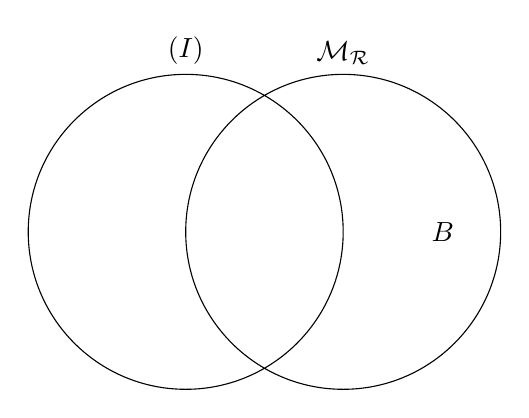
\begin{tikzpicture}
          \draw (-1, 0 ) circle (2)
                (-1, 2 ) node [above] {$\LT(I)$}
                ( 1, 0 ) circle (2)
                ( 1, 2 ) node [above] {$\cal M_R$}
                ( 2, 0 ) node [right] {$B$};
        \end{tikzpicture}
      \end{center}
      
      Either $\LT(f) \in B$ or $\LT(f) \in \LT(I)$.
      In the first case, suppose $\LT(f) = b \in B$.
      Then $f - b \in R - X$ has a smaller leading term than $f$,
      contradicting our choice of $f$.
      Otherwise, suppose $\LT(f) = m \in \LT(I)$.
      Then we can subtract from $f$ any monic polynomial in $I$ with the same leading term,
      again yielding a smaller polynomial in $R - X$.
  \end{description}
\end{proof}
\end{comment}

\begin{corollary}
  \label{cor_dim_R_mod_I}
  $$\dim_K R/I = \#\{ m \in \cal M_R ~|~ m \not\in \LT(I)\}.$$
\end{corollary}
\begin{theorem}
  Let $G = \{g_1, \ldots, g_m\}$ be a Gr\"obner basis and consider the system of polynomial equations
  \[g_1 = \ldots = g_m = 0.\]
  This system has finitely many solutions if and only if for every indeterminate $x_i \in K[x_1, \ldots, x_n]$,
  there is a power $x_i^k$ and element $g \in G$ such that $\LM(g) = x_i^k$.
\end{theorem}
\begin{proof}
  \S 3.6 of \cite{buchberger98}.
\end{proof}

\begin{theorem}
  Let $G = \{g_1, \ldots, g_m\}$ be a Gr\"obner basis and suppose the system of polynomial equations
  \[g_1 = \ldots = g_m = 0\]
  has finitely many solutions.
  Let $N$ be the number of solutions.
  \begin{enumerate}[label=(\roman*)]
    \item $N = \#\{ m \in \cal M_R ~|~ m \not\in \pid{\LT(g_1), \ldots, \LT(g_m)} \}$.
    \item If $I$ is the $R$-ideal generated by $G$, then $N = \dim_K R/I$.
  \end{enumerate}
\end{theorem}
\begin{proof}
  For part (i), see \S 3.6 of \cite{buchberger98}.
  Part (ii) follows from Corollary \ref{cor_dim_R_mod_I}.
\end{proof}
\begin{comment}
\begin{theorem}
  \label{thm_groebner_basis_product}
  Let $I$ and $J$ be ideals of $R = K[x_1, \ldots, x_n]$, generated by Gr\"obner bases, say
  \begin{align*}
    I &= \pid{f_1, \ldots, f_m} \\
    J &= \pid{g_1, \ldots, g_n}.
  \end{align*}
  Then
  \[ \{ f_ig_j ~|~ 1 \leq i \leq m, 1 \leq j \leq n \} \]
  is a Gr\"obner basis for the ideal product $IJ$.
\end{theorem}
\begin{proof}
  \begin{align*}
    \LT(IJ)
      &= \pid{ \LT(h) ~|~ h \in IJ } \\
      &= \pid{ \LT(fg) ~|~ f \in I, g \in J } \\
      &= \pid{ \LT(f)\LT(g) ~|~ f \in I, g \in J } \\
      &= \pid{ \LT(f) ~|~ f \in I } \pid{ \LT(g) ~|~ g \in J } \\
      &= \LT(I) \LT(J) \\
      &= \pid{ \LT(f_i) ~|~ 1 \leq i \leq m } \pid{ \LT(g_j) ~|~ 1 \leq j \leq n } \\
      &= \pid{ \LT(f_i) \LT(g_j) ~|~ 1 \leq i \leq m, 1 \leq j \leq n } \\
      &= \pid{ \LT(f_i g_j) ~|~ 1 \leq i \leq m, 1 \leq j \leq n }
  \end{align*}
\end{proof}
\end{comment}

\begin{theorem}
  \label{thm_groebner_basis_remainder}
  Let $I$ be an ideal of $R$, generated by the Gr\"obner basis $G = \{ g_1, \ldots, g_m \}$. Then
  \begin{enumerate}[label=(\roman*)]
    \item
    Every polynomial $f \in R$ can be written uniquely in the form
    \begin{equation*}
      f = g + r
    \end{equation*}
    where $g \in I$, $r \in R$, and $r$ is reduced modulo $G$.

    \item
    For any polynomial $f \in R$, we have that $f \in I$ if and only if $r = 0$.
  \end{enumerate}
\end{theorem}
\begin{proof}
  Chapter 2, \S 6, Proposition 1 and Corollary 2 in \cite{cox07}.
\end{proof}

\begin{comment}
It is an obvious fact that, given any polynomial $f \in K[x_1, \ldots, x_n]$,
we can separate $f$ into its homogeneous components.
That is, we can write
\[ f = \sum_{i = 0}^n f_i^* \]
where $n$ is the total degree of $f$ and $f_i^*$ is homogeneous of degree $i$.

Given a point $P = (a_1, \ldots, a_n) \in \bb A_K^n$, we can even write $f$ in the same form,
but where $f_i^*$ is homogeneous in the variables $(x_1 - a_1), \ldots, (x_n - a_n)$.
E.g., in $\bb Q[x,y]$, given the point $P = (1,1)$, 
\[ x^2 + y^2 = [(x - 1)^2 + (y - 1)^2] + [2(x + 1) + 2(y + 1)] + [2]. \]
This is just the multivariate Taylor series expansion of the polynomial around the point $P$.
This generalizes to the following.

\begin{theorem}
  Let $R = K[x_1, \ldots, x_n]$ and let $I$ be an ideal of $R$ given by a Gr\"obner basis $I = \pid{g_1, \ldots, g_m}$.
  Then $f$ can be written uniquely in the form
  \[ f = \sum_{i=0}^t f_i^*, \]
  where $t = \max\{n \in \bb N ~|~ f \in I^n\}$, $f_i^* \in I^i - I^{i+1}$, and $f_i^* \not\in \LT(I^{i+1})$.
\end{theorem}
\begin{proof}
  By Theorem \ref{thm_groebner_basis_product}, our Gr\"obner basis for $I$ gives us a basis for $I^t$.
  Theorem \ref{thm_groebner_basis_remainder} then applies, allowing us to write
  \[ f = f^*_t + r_t \]
  with $f^*_t \in I^t - I^{t+1}$ and $r_t \in R$, $r_t \not\in \LT(I^t)$.
  Applying Theorems \ref{thm_groebner_basis_product} and \ref{thm_groebner_basis_remainder} $t-1$ more times gives the result.
\end{proof}

Essentially, given finitely polynomials $\{ g_i \}$ forming a Gr\"obner basis for an ideal,
we can uniquely perform a homogenous decomposition of any polynomial $f$ with respect to the $g_i$'s.

This also allows us to show that (over a field of sufficiently large characteristic)
$f \in I^2$ if and only if $f$ and its differential $df$ vanish modulo $I$.
\end{comment}



%%%%%%%%%%%%%%%%%%%%%%%%%%%%%%%%%%%%%%%%%%%%%%%%%%
%%%%%                                        %%%%%
%%%%%   Groebner Bases in Coordinate Rings   %%%%%
%%%%%                                        %%%%%
%%%%%%%%%%%%%%%%%%%%%%%%%%%%%%%%%%%%%%%%%%%%%%%%%%

\subsection{Gr\"obner Bases in Coordinate Rings}

While the theory of Gr\"obner bases always takes place in polynomial rings,
in Chapter \ref{chap_representation}, we will speak of Gr\"obner bases for ideals of a coordinate ring,
which is the quotient of a polynomial ring by a prime ideal (see Definition \ref{def_coordinate_ring}).
We make clear here what is meant by that.

Let $R = K[x,y]$ be a bivariate polynomial ring and $f \in R$ be irreducible over $K$.
Let $K[C] = R/\pid f$.
Then the ideals of $R$ containing $f$ are in bijection with the ideals of $K[C]$
(Theorem III.2.13 in \cite{hungerford}).
Let $G = \pid{g_1, \ldots, g_m}$ be a finite subset of $K[C]$
and let $I = \pid G$ be the $K[C]$-ideal generated by $G$.
Let $\bar f \in R$ be the reduction of $f \in R$ modulo $G$, in the sense of Definition \ref{def_reduced_polynomial},
and treating $G$ as a subset of $R$.
We will say that $G$ is a Gr\"obner basis for $I$ if the set $G \cup \{ \bar f \}$ is a Gr\"obner basis in $K[x,y]$.

In each of the examples below,
let $K = \bb F_{11}$,
let $R = K[x,y]$ with the $C_{3,4}$ order,
and let $f = y^3 + x^4 + 1$ and $K[C] = R/\pid f$.
\begin{example}
  Consider the ideal $I = \pid{x^2 + x, xy} \subset K[C]$.
  The set $\{ x^2 + x, xy \}$ is \emph{not} a Gr\"obner basis.
  The reduction of $f$ modulo its generators is $\bar f = y^3 - x + 1$.
  Now we lift $I$ to $I^* = \pid{x^2 + x, xy, y^3 - x + 1} \subset R$.
  However, one of the $S$-polynomials of the generators of $I^*$ does not reduce to 0.
  \begin{align*}
    S(x^2 + x, y^3 - x + 1)
      &= (x^2 + x)\frac{x^2y^3}{x^2} - (y^3 - x + 1)\frac{x^2y^3}{y^3} \\
      &= xy^3 + x^3 - x^2 \\
      &\equiv x^3 - x^2 \\
      &\equiv 2x.
  \end{align*}
  By contrast, $\{x^2 + x, xy\}$ \emph{is} a Gr\"obner basis of $K[x,y]$,
  as per Example \ref{ex_groebner_2}.
\end{example}
\begin{example}
  Consider instead $I = \pid{y^2} \subset K[C]$.
  The reduction of $f$ modulo $y^2$ is $\bar f = x^4 + 1$.
  Lift $I$ to $I^* = \pid{y^2, x^4 + 1} \subset R$.
  The $S$-polynomial $S(y^2, \bar f) = y^2 \equiv 0$,
  hence $\{y^2\}$ is a Gr\"obner basis in $K[C]$.
\end{example}
